% Einsum Trees — ASPLOS 2025 — Beamer Slide Deck
% Compile with: pdflatex einsum_trees_slides.tex (twice for references)
% Requires: beamer, tikz, booktabs, listings

\documentclass[aspectratio=169,10pt]{beamer}

\usepackage[T1]{fontenc}
\usepackage[utf8]{inputenc}
\usepackage{lmodern}
\usepackage{tikz}
\usetikzlibrary{shapes.geometric,arrows.meta,positioning,calc,fit}
\usepackage{booktabs}
\usepackage{listings}
\usepackage{array}
\usepackage{colortbl}
\usepackage{xcolor}
\usepackage{graphicx}

% ─── Colors ───────────────────────────────────────────────────────────────────
\definecolor{Navy}{RGB}{28,45,80}
\definecolor{Crimson}{RGB}{155,34,38}
\definecolor{Gold}{RGB}{181,98,26}
\definecolor{Forest}{RGB}{26,102,52}
\definecolor{CodeBg}{RGB}{229,225,216}
\definecolor{ScratchBg}{RGB}{255,253,231}
\definecolor{PlaceholderBg}{RGB}{229,225,216}

% ─── Theme ────────────────────────────────────────────────────────────────────
\usetheme{metropolis}

\setbeamercolor{alerted text}{fg=Crimson}
\setbeamercolor{example text}{fg=Forest}

% ─── Helpers ──────────────────────────────────────────────────────────────────
\newcommand{\ein}[1]{{\small\texttt{#1}}}
\newcommand{\einl}[1]{{\footnotesize\texttt{#1}}}
\newcommand{\code}[1]{{\small\texttt{\colorbox{CodeBg}{\textcolor{Navy}{#1}}}}}

% Scratch-paper block
\newenvironment{scratch}{%
  \setbeamercolor{block title}{fg=black!70,bg=ScratchBg!80!yellow}
  \setbeamercolor{block body}{bg=ScratchBg}
  \begin{block}{}
  \footnotesize\ttfamily
}{%
  \end{block}
}

% Image placeholder
\newcommand{\imgplaceholder}[2][5cm]{%
  \begin{tikzpicture}
    \node[draw=gray,dashed,fill=PlaceholderBg,rounded corners=3pt,
          minimum width=\linewidth,minimum height=#1,align=center,text=gray!70,
          font=\footnotesize] {#2};
  \end{tikzpicture}
}

% TikZ tree styles
\tikzset{
  tnode/.style={rectangle,rounded corners=3pt,draw=Navy,fill=white,
                font=\footnotesize\ttfamily,minimum width=1.0cm,minimum height=.45cm,
                inner sep=2pt},
  tleaf/.style={tnode,fill=CodeBg},
  topt/.style={tnode,draw=Forest,fill=Forest!10},
  tedge/.style={->,>=Stealth,Navy,thick},
}

% ─── Document ─────────────────────────────────────────────────────────────────
\title{Einsum Trees}
\subtitle{An Abstraction for Optimizing the Execution of Tensor Expressions}
\author{Breuer · Blacher · Engel · Giesen · Heinecke · Klaus · Remke\\}
\date{CS259::Paul Talma\\\today}

\begin{document}

% ─── S1: TITLE ────────────────────────────────────────────────────────────────
\begin{frame}
\maketitle
\textit{[Your name] \quad [Course name]}
\end{frame}

% ─── TABLE OF CONTENTS ────────────────────────────────────────────────────────
\begin{frame}{Overview}
\tableofcontents
\end{frame}

\section{Einsum Notation}

% ─── S2: EINSUM NOTATION ──────────────────────────────────────────────────────
\begin{frame}{Einsum Notation}
	Einsum notation is a compact notation for \textbf{pure tensor operations}.

	Canonical form:
\begin{center}
\ein{einsum($I_1, \ldots, I_n \to O\,;\, T_1, \ldots, T_n$)}	
\end{center}	
	
	
\end{frame}

\begin{frame}{Einsum Notation}

A compact notation for \textbf{pure tensor operations}:

\begin{center}
\ein{einsum($I_1, \ldots, I_n \to O\,;\, T_1, \ldots, T_n$)}	
\end{center}

Examples:
%\begin{itemize}
%	\item \einl{einsum(pq, qr -> pr); A, B)}
%\end{itemize}

\begin{center}
\begin{tabular}{@{}l@{\quad}l@{}@{\quad}l@{}}
\toprule
\textbf{Expression} & \textbf{Operation} & \textbf{Name} \\
\midrule
\einl{einsum(pq, qr -> pr; A, B)} & $O_{pr} = \sum_{q} A_{pq}B_{qr}$ & Matrix multiply $A \cdot B$ \\
\einl{einsum(pq, pq -> pq; A, B)} & $O_{pq} = A_{pq}B_{pq}$ & Hadamard product $A \odot B$ \\
\einl{einsum(pq, qr -> r; A, B)} & $O_{r} = \sum_{pq}A_{pq}B_{qr}$ & $= \sum_q B_{qr} \sum_p A_{pq}$\\
%\einl{einsum(pq, qr -> pqr; A, B)} & Khatri-Rao product \\
%\einl{einsum(pq, rs -> pqrs; A, B)} & Kronecker product \\
\bottomrule
\end{tabular}	
\end{center}

Rough semantics: indices in inputs but not outputs are contracted (sum-of-products).

\end{frame}

\begin{frame}{Attractions of Einsum}
	\begin{columns}
		\begin{column}{0.3\textwidth}
				Concise
				
				Literate
				
				Efficient
		\end{column}
	
		\begin{column}{0.7\textwidth}
			\begin{figure}
				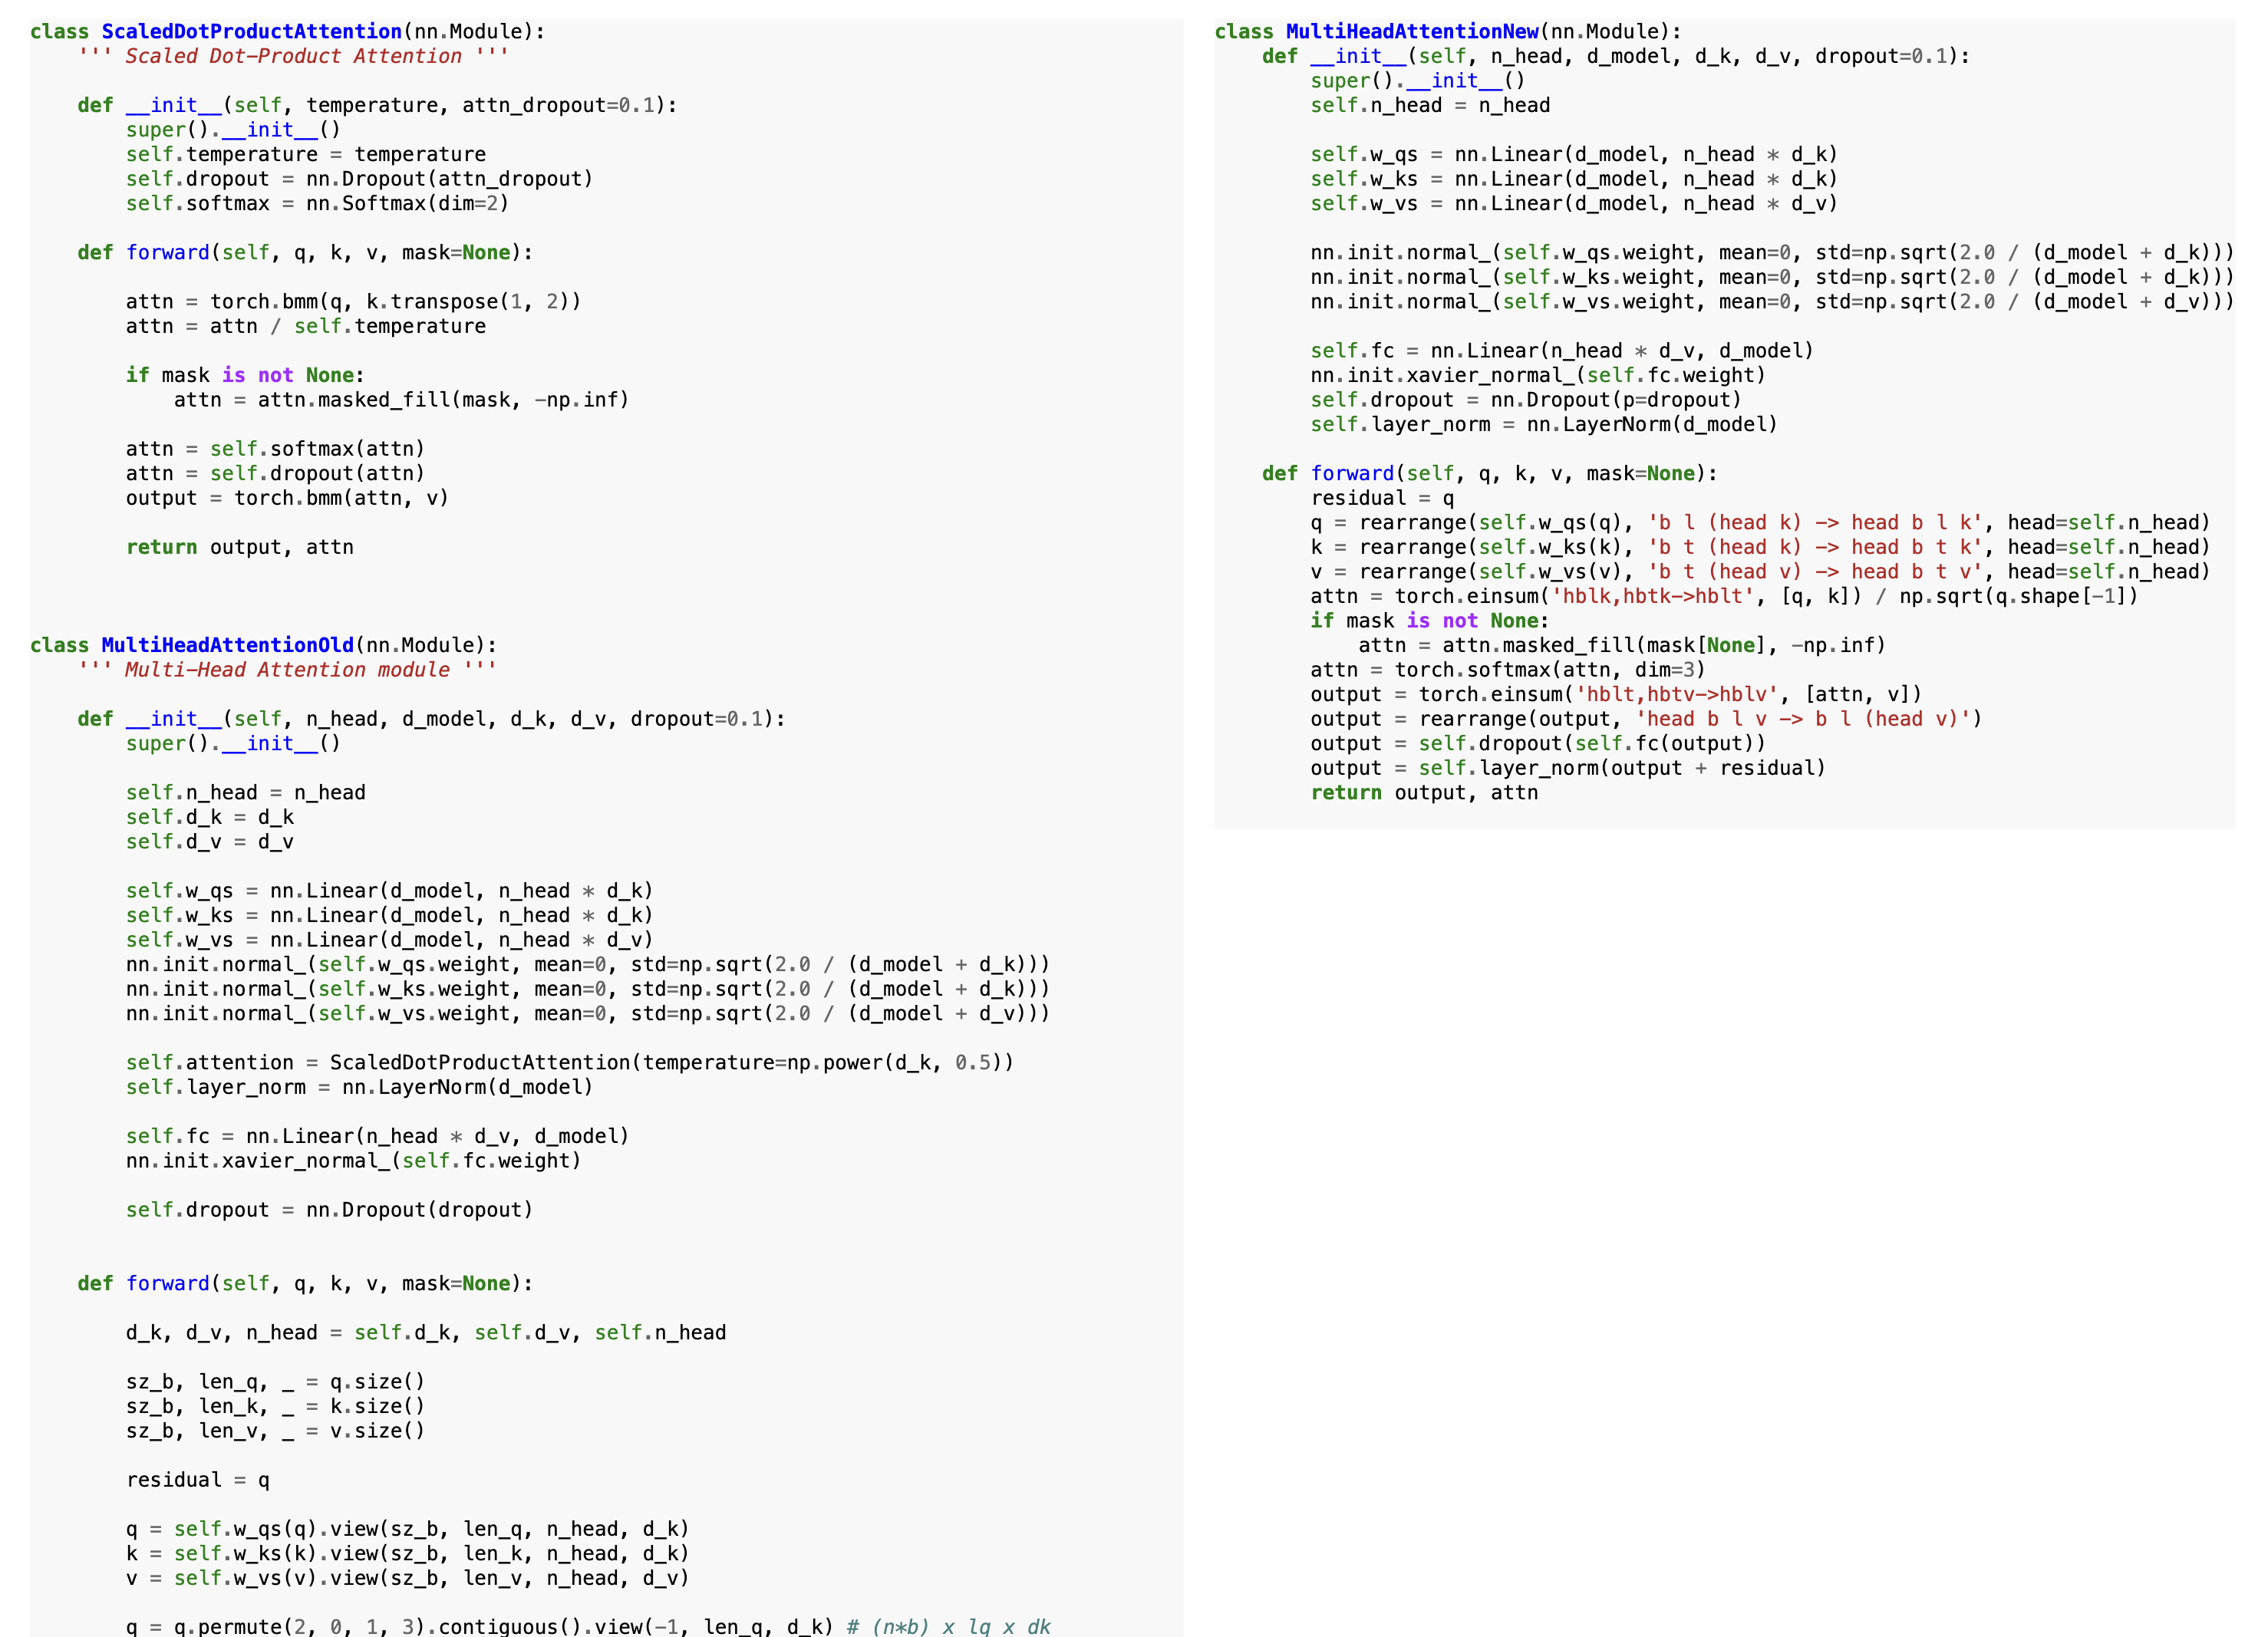
\includegraphics[width=\linewidth]{comparison}
			\end{figure}	
		\end{column}
	\end{columns}
\end{frame}

\begin{frame}{The Problem}
	Einsum notation specifies what to compute, not how.
	
	Different implementations vary widely in their efficiency.
	
	How can we efficiently compile einops into efficient implementations?
	
\end{frame}


% ─── S3: CONTRACTION PATHS ────────────────────────────────────────────────────
\begin{frame}{Contraction Paths}

\begin{columns}[T]
\column{.50\textwidth}
\begin{itemize}
  \item An $n$-ary einsum decomposes into binary contractions
  \item Different orderings: same result, different flop counts/max intermediate tensor size
  \item Finding the optimal path is \alert{NP-hard}.
        Good heuristics exist: cotengra, opt\_einsum
  \item The chosen schedule is the \textbf{contraction path}
\end{itemize}

\pause
\column{.48\textwidth}
\einl{einsum(pq,qr,rs,st->pt; A,B,C,D)}

\medskip
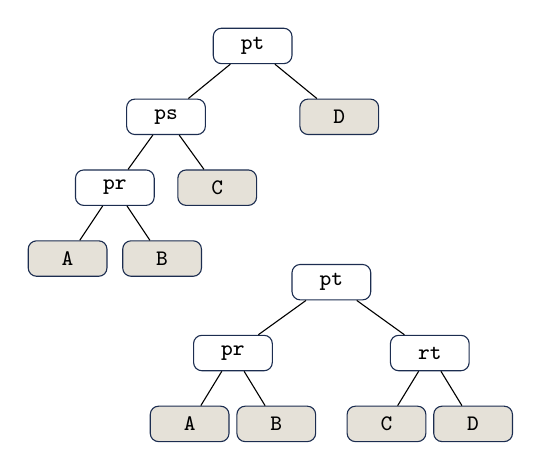
\begin{tikzpicture}[level distance=0.9cm,
    level 1/.style={sibling distance=2.2cm},
    level 2/.style={sibling distance=1.3cm},
    level 3/.style={sibling distance=1.2cm}]
  \node[tnode] {pt}
    child { node[tnode] {ps}
      child { node[tnode] {pr}
        child { node[tleaf] {A} }
        child { node[tleaf] {B} }
      }
      child { node[tleaf] {C} }
    }
    child { node[tleaf] {D} };
  %
  \begin{scope}[yshift=-3cm,
  xshift=1cm,
      level 1/.style={sibling distance=2.5cm},
      level 2/.style={sibling distance=1.1cm}]
    \node[tnode] {pt}
      child { node[tnode] {pr}
        child { node[tleaf] {A} }
        child { node[tleaf] {B} }
      }
      child { node[tnode] {rt}
        child { node[tleaf] {C} }
        child { node[tleaf] {D} }
      };
  \end{scope}
\end{tikzpicture}

\end{columns}
\end{frame}

%\begin{frame}{Contraction Paths (cont.)}
%	Symbolically:
%	\begin{align*}
%	&\ \code{einsum(pq,qr,rs,st->pt; A, B, C, D)}\\
%	\equiv &\ \code{einsum(pr,rs,st->pt; einsum(pq,qr->pr; A, B), C, D)}\\
%	\equiv &\ \code{einsum(ps,st->pt; einsum(pr,rs->ps; einsum(pq,qr->pr; A, B), C), D)}
%	\end{align*}
%
%\end{frame}

% ─── S4: TPPs ─────────────────────────────────────────────────────────────────
\begin{frame}{Tensor Processing Primitives (TPPs)}

A small set of hand-optimized kernels.

The main primitive is GEMM: 
\code{C[N][M] += A[K][M] * B[N][K]}.
(Also: batched (``packed'') GEMM,  transpose.)

\medskip
\begin{itemize}
  \item Efficient because: cache-blocked tiling keeps the working set in L1/L2,
        SIMD vectorizes the inner $K$ loop, register reuse amortizes memory latency
  \item Requires K, M, N to be \textbf{rightmost in memory}.
        Row-major storage: last index in the index string is the unit-stride (fast) dimension
  \item Loop dimensions outside the GEMM are iterated with OpenMP.
        Must be large enough to saturate cores, small enough to keep the GEMM tile in cache
\end{itemize}
\end{frame}

\section{Motivation}

% ─── S5: THE JOINT PROBLEM ────────────────────────────────────────────────────
\begin{frame}{Two Problems, Solved in Isolation}

\begin{columns}[T]
\column{.46\textwidth}
\textbf{\color{Navy}Contraction path optimization}
\begin{itemize}
  \item Minimizes flops or peak intermediate size
  \item Assumes fixed row-major layout, ignores data movement
\end{itemize}

\column{.46\textwidth}
\textbf{\color{Navy}Local binary lowering}
\begin{itemize}
  \item Optimizes layout for one contraction at a time
  \item Unaware of the layout produced by the preceding step
\end{itemize}
\end{columns}

\bigskip\hrule\bigskip

\begin{block}{Consequence}
\centering
Unnecessary tensor transpositions between contractions.\\
A full memory read and write per contraction step.
\end{block}

\bigskip
\centering
\textcolor{Crimson}{\bfseries Joint optimization over the full contraction path is the opportunity.}
\end{frame}

% ─── S6: WHAT GOES WRONG ──────────────────────────────────────────────────────
\begin{frame}{What Goes Wrong Without Joint Optimization}

\begin{columns}[T]
\column{.44\textwidth}
Task: \einl{einsum(pq, qr, rs -> ps)}, path $(A \cdot B) \cdot C$

\medskip
\textcolor{Crimson}{\bfseries Local (isolated) approach:}
\begin{itemize}
  \item Step 1: optimize $A \cdot B$ locally.
        Natural output layout: \ein{pr} ($p{=}M$, $r{=}N$, $q{=}K$).
  \item Step 2: need \einl{einsum(pr, rs -> ps)}.\\
        $K{=}r$ must be rightmost in $I_1$. Have \ein{pr}. Need \ein{rp}.
        \alert{Transpose required.}
\end{itemize}

\medskip
\textcolor{Forest}{\bfseries Joint approach:}
\begin{itemize}
  \item Step 1 produces layout \ein{rp} instead.
  \item Step 2: $I_1 = \texttt{rp}$.
        Condition satisfied. \textcolor{Forest}{No transpose.}
\end{itemize}

\column{.53\textwidth}
\begin{scratch}
Step 2 GEMM condition:

  I1 must end with KM.
  K = r, M = p.

  Local result:  I1 = pr  <- wrong order
  Transpose:        pr -> rp  <- full memory pass

  Joint result:  I1 = rp  <- correct order
  No transpose needed.             ok

Cost of one transposition:
  O(|p| * |r|) memory reads+writes.
  Paid at every contraction step
  if layouts are chosen in isolation.
\end{scratch}
\end{columns}
\end{frame}

\section{The Einsum Trees Solution}

% ─── S7: CONTRIBUTIONS ────────────────────────────────────────────────────────
\begin{frame}{Main Contributions}

\begin{block}{Einsum Tree IR}
\medskip
An intermediate representation encoding both the contraction path and the memory
layout of every intermediate tensor, globally.
\end{block}

\medskip
\begin{block}{Optimization algorithm}
\medskip
Three simple tree transformations applied in a single deterministic preorder traversal.
No search, no autotuning. Compile time under 4\,ms.
\end{block}

\medskip
\begin{block}{\texttt{einsum\_ir}: open-source C++ implementation}
\medskip
Backend: LIBXSMM + OpenMP. MIT license.
Evaluated on Arm (Grace), x86 server (Xeon), x86 desktop (Ryzen).
\end{block}
\end{frame}

% ─── S8: SOLUTION OVERVIEW ────────────────────────────────────────────────────
\begin{frame}{How the Pieces Fit Together}

\begin{center}
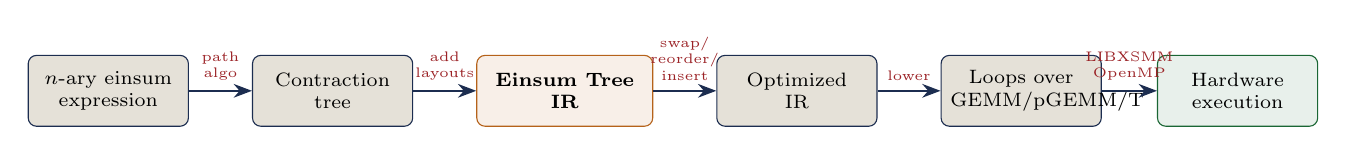
\begin{tikzpicture}[node distance=0.55cm and 0.5cm,
    box/.style={rectangle,rounded corners=3pt,draw=Navy,fill=CodeBg,
                font=\scriptsize,minimum height=0.9cm,text width=1.8cm,align=center},
    hl/.style={rectangle,rounded corners=3pt,draw=Gold,fill=Gold!10,
               font=\scriptsize\bfseries,minimum height=0.9cm,text width=2.0cm,align=center},
    arr/.style={->,>=Stealth,Navy,thick},
    lbl/.style={font=\tiny,color=Crimson,align=center}]

  \node[box] (ein) {$n$-ary einsum\\expression};
  \node[box, right=0.8cm of ein] (ctree) {Contraction\\tree};
  \node[hl,  right=0.8cm of ctree] (ir) {Einsum Tree\\IR};
  \node[box, right=0.8cm of ir] (opt) {Optimized\\IR};
  \node[box, right=0.8cm of opt] (low) {Loops over\\GEMM/pGEMM/T};
  \node[box, right=0.7cm of low, draw=Forest, fill=Forest!10] (exec) {Hardware\\execution};

  \draw[arr] (ein) -- (ctree)   node[lbl,above,midway]{path\\algo};
  \draw[arr] (ctree) -- (ir)    node[lbl,above,midway]{add\\layouts};
  \draw[arr] (ir) -- (opt)      node[lbl,above,midway]{swap/\\reorder/\\insert};
  \draw[arr] (opt) -- (low)     node[lbl,above,midway]{lower};
  \draw[arr] (low) -- (exec)    node[lbl,above,midway]{LIBXSMM\\OpenMP};
\end{tikzpicture}
\end{center}

\medskip
\begin{itemize}
  \item The IR gives the optimizer a \textbf{global view} of layout decisions across the full contraction path
  \item Both optimization and lowering are deterministic single-pass algorithms. No tuning loop.
  \item Dimension taxonomy (R/C/M/N/K) governs the lowering at every node
\end{itemize}
\end{frame}

% ─── S9: DIMENSION TAXONOMY ───────────────────────────────────────────────────
\begin{frame}{Dimension Taxonomy}

\begin{tabular}{@{}llll@{}}
\toprule
\textbf{Type} & \textbf{Appears in} & \textbf{Role} & \textbf{Example (einsum(pq,qr$\to$pr))} \\
\midrule
\textcolor{Navy}{\bfseries K} & Both inputs, not output & GEMM $K$ (contraction) & $q$ \\
\textcolor{Navy}{\bfseries M} & Left input + output & GEMM $M$ & $p$ \\
\textcolor{Navy}{\bfseries N} & Right input + output & GEMM $N$ & $r$ \\
\textcolor{Navy}{\bfseries C} & Both inputs + output & Packed GEMM batch dim & $p$ in \einl{einsum(pqr,psr->pqs)} \\
\textcolor{Navy}{\bfseries R} & One input, not output & Unary reduction & $q$ in \einl{einsum(pq,p->p)} \\
\bottomrule
\end{tabular}

\bigskip
\begin{itemize}
  \item Dimensions not mapped to a GEMM type become \textbf{loop dimensions}: iterated with OpenMP
  \item Key constraint: K, M, N, C must occupy the \alert{rightmost positions} in each index string
\end{itemize}
\end{frame}

% ─── S10: EINSUM TREE IR ──────────────────────────────────────────────────────
\begin{frame}{Einsum Tree IR}

\begin{columns}[T]
\column{.55\textwidth}
\textbf{Contraction tree (baseline):}
\begin{itemize}
  \item Rooted binary tree. Leaves: input tensors. Root: output.
  \item Encodes contraction order, abstracts irrelevant details
\end{itemize}

\medskip
\textbf{Einsum Tree IR adds:}
\begin{itemize}
  \item \textcolor{Navy}{\bfseries Dimension ordering} at each node.
        The index string \emph{is} the memory layout declaration.
  \item Each dimension labeled K/M/N/C/loop
  \item Unary nodes for \textcolor{Navy}{\bfseries permutations} (transpose primitive)
\end{itemize}

\column{.42\textwidth}
\begin{center}
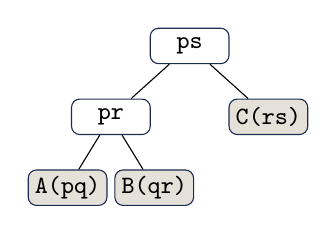
\begin{tikzpicture}[level distance=0.9cm,
    level 1/.style={sibling distance=2.0cm},
    level 2/.style={sibling distance=1.1cm}]
  \node[tnode] {\ein{ps}}
    child { node[tnode] {\ein{pr}}
      child { node[tleaf] {\ein{A(pq)}} }
      child { node[tleaf] {\ein{B(qr)}} }
    }
    child { node[tleaf] {\ein{C(rs)}} };
\end{tikzpicture}

\smallskip
{\footnotesize\einl{einsum(pq, qr, rs -> ps)}}
\end{center}
\end{columns}
\end{frame}

% ─── S11: GEMM MAPPING CONDITION ──────────────────────────────────────────────
\begin{frame}{GEMM Mapping Condition}

For binary node \ein{einsum($I_1$, $I_2$ $\to$ $O$)} to map to a (packed) GEMM:

\bigskip
\begin{block}{}
\centering
\begin{tabular}{rl}
$I_1$ : & $\ldots\;\textcolor{Gold}{g_K}\;\textcolor{Navy}{g_M}\;\textcolor{Crimson}{g_C}$ \\[4pt]
$I_2$ : & $\ldots\;\textcolor{Navy}{g_N}\;\textcolor{Gold}{g_K}\;\textcolor{Crimson}{g_C}$ \\[4pt]
$O$   : & $\ldots\;\textcolor{Navy}{g_N}\;\textcolor{Navy}{g_M}\;\textcolor{Crimson}{g_C}$ \\
\end{tabular}
\end{block}

\medskip
{\small $g_K, g_M, g_N$: contiguous blocks of K/M/N-type dims. $g_C$: batch dims.}

\bigskip
\begin{itemize}
  \item Remaining dims become \textbf{loop dimensions}, parallelized with OpenMP
  \item When the mapping fails, a \textbf{transpose} node is inserted.
        The optimizer's goal: satisfy this condition at every node without unnecessary transpositions
\end{itemize}
\end{frame}

% ─── S12: OPTIMIZATION ALGORITHM ─────────────────────────────────────────────
\begin{frame}{Optimizing Einsum Trees}

\begin{columns}[T]
\column{.50\textwidth}
\textbf{Three transformations:}
\begin{itemize}
  \item \textbf{Swap.} Exchange left and right children
  \item \textbf{Reorder.} Permute the index string at a node
  \item \textbf{Insert.} Add a unary permutation node (transpose primitive)
\end{itemize}

\medskip
\textbf{Procedure:}
\begin{itemize}
  \item Preorder traversal. At each binary node: classify dims, apply transformations until GEMM mapping satisfied
  \item Leaf mismatches realized as transpose primitives
\end{itemize}

\column{.47\textwidth}
\begin{block}{No search required}
Transformations applied greedily at each node.
Single pass over the tree.
\end{block}

\medskip
\textbf{Compile time:}

\smallskip
\begin{tabular}{@{}ll@{}}
\toprule
Approach & Time \\
\midrule
ET-TPP (this work) & \textbf{$<$4 ms} \\
ET-TBLIS            & $<$2 ms \\
OE-Torch            & $<$1 ms \\
TVM-Ansor           & \alert{$10^3$--$10^4$ s} \\
\bottomrule
\end{tabular}
\end{columns}
\end{frame}

% ─── S13: TOY EXAMPLE PART 1 ──────────────────────────────────────────────────
\begin{frame}{Toy Example: Initial Tree and Root Analysis}

\begin{columns}[T]
\column{.38\textwidth}

\einl{einsum(pq, qr, rs -> ps)}, path $(A \cdot B) \cdot C$

\medskip
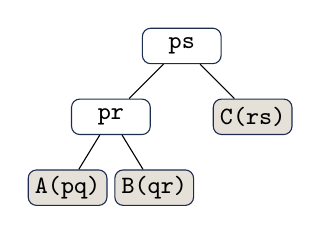
\begin{tikzpicture}[level distance=0.9cm,
    level 1/.style={sibling distance=1.8cm},
    level 2/.style={sibling distance=1.1cm}]
  \node[tnode] {\ein{ps}}
    child { node[tnode] {\ein{pr}}
      child { node[tleaf] {\ein{A(pq)}} }
      child { node[tleaf] {\ein{B(qr)}} }
    }
    child { node[tleaf] {\ein{C(rs)}} };
\end{tikzpicture}

\column{.58\textwidth}
\begin{scratch}
Root node: einsum(pr, rs -> ps)

Classify dims:
  p: left + output only -> M
  r: both inputs, not output -> K
  s: right + output only -> N

GEMM condition needs:
  I1 ends with KM = rp  (have: pr)  x
  I2 ends with NK = sr  (have: rs)  x
  O  ends with NM = sp  (have: ps)  x

-> Reorder all three index strings.
\end{scratch}
\end{columns}
\end{frame}

% ─── S14: TOY EXAMPLE PART 2 ──────────────────────────────────────────────────
\begin{frame}{Toy Example: Optimized Tree}

\begin{columns}[T]
\column{.38\textwidth}

After full optimization:

\medskip
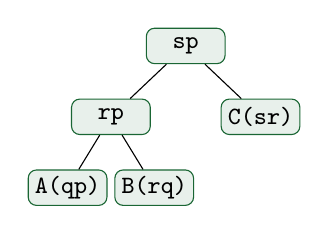
\begin{tikzpicture}[level distance=0.9cm,
    level 1/.style={sibling distance=1.9cm},
    level 2/.style={sibling distance=1.1cm}]
  \node[topt] {\ein{sp}}
    child { node[topt] {\ein{rp}}
      child { node[topt] {\ein{A(qp)}} }
      child { node[topt] {\ein{B(rq)}} }
    }
    child { node[topt] {\ein{C(sr)}} };
\end{tikzpicture}

\column{.58\textwidth}
\begin{scratch}
Recurse into child: einsum(qp, rq -> rp)

  p: M,  q: K,  r: N

  I1 ends with KM = qp  ok
  I2 ends with NK = rq  ok
  O  ends with NM = rp  ok

Child output rp = root's I1 requirement.
No transpose node needed anywhere.  ok
\end{scratch}

\medskip
\begin{itemize}
  \item \texttt{rp} satisfies the child's GEMM condition \emph{and} the parent's $I_1$ requirement simultaneously
  \item Local approach: produces \texttt{pr}, forces a transpose at the next step
\end{itemize}
\end{columns}
\end{frame}

\section{Evaluation}

% ─── S15: RESULTS SINGLE CONTRACTIONS ────────────────────────────────────────
\begin{frame}{Results: Single Binary Contractions (TCCG)}

\begin{columns}[T]
\column{.50\textwidth}
\imgplaceholder[3.5cm]{[ Insert Fig.\ 3 from paper ]\\Grace testbed: GFLOPS vs.\ TCCG setting ID\\ET-TPP $\cdot$ ET-TBLIS $\cdot$ TVM-Ansor $\cdot$ ATen $\cdot$ OE-Torch}

\column{.47\textwidth}
\begin{itemize}
  \item 24 benchmark settings. ET-TPP competitive across all three testbeds.
  \item TVM-Ansor slightly ahead on a subset, but requires \alert{hours of autotuning} vs. milliseconds for ET-TPP.
  \item Settings 17--18: small loop dimensions limit OpenMP parallelism. A known weakness of the greedy heuristic.
  \item ATen and OE-Torch (TTGT-style local lowering) are consistently slower. The gap quantifies avoided transposition overhead.
\end{itemize}
\end{columns}
\end{frame}

% ─── S16: RESULTS CONTRACTION TREES ──────────────────────────────────────────
\begin{frame}{Results: Complex Contraction Trees}

\begin{columns}[T]
\column{.50\textwidth}
{\small Grace testbed, FP32 GFLOPS}

\smallskip
\begin{tabular}{@{}llll@{}}
\toprule
\textbf{Workload} & \textbf{ET-TPP} & \textbf{Best other} & \textbf{Speedup} \\
\midrule
SYN  & 4838 & 3172 (Ansor)  & \textbf{1.5$\times$} \\
TT   & 3315 & 2455 (TBLIS)  & \textbf{1.4$\times$} \\
FCTN & 3092 & 2578 (Ansor)  & \textbf{1.2$\times$} \\
TRN  & 1963 & 933 (TBLIS)   & \textcolor{Crimson}{\bfseries 2.1$\times$} \\
MERA & 4025 & 1958 (TBLIS)  & \textcolor{Crimson}{\bfseries 2.1$\times$} \\
TNLM & 4378 & 3532 (Torch)  & \textbf{1.4$\times$} \\
\bottomrule
\end{tabular}

\imgplaceholder[1.5cm]{[ Insert Figs.\ 3--5 for full per-testbed plots ]}

\column{.47\textwidth}
\begin{itemize}
  \item ET-TPP outperforms all four baselines on most workloads.
  \item TVM-Ansor: \alert{N/A for MERA, TNLM}. OOM or timeout after 12 hours.
  \item TW on SPR: ET-TBLIS wins. Small $h$-dimension limits vectorization.
\end{itemize}
\end{columns}
\end{frame}

\section{Discussion}

% ─── S17: CRITICAL EVALUATION ────────────────────────────────────────────────
\begin{frame}{Critical Evaluation}

\begin{columns}[T]
\column{.48\textwidth}
\textcolor{Crimson}{\bfseries Comparison to TTGT}

\begin{itemize}\small
  \item TTGT (used by ATen, partially by OE-Torch): permute inputs to GEMM layout, call GEMM, permute output back. Always pays 2--3 transpositions per contraction.
  \item ET-TPP's advantage is exactly the elimination of these transpositions. The speedup over ATen/OE-Torch directly quantifies this benefit.
\end{itemize}

\medskip
\textcolor{Crimson}{\bfseries TVM-Ansor}

\begin{itemize}\small
  \item Ansor searches a larger space. ET-TPP beats it anyway on most settings.
  \item Ansor is unusable for MERA and TNLM (OOM/timeout). ET-TPP compiles both in under 10\,ms.
\end{itemize}

\column{.48\textwidth}
\textcolor{Crimson}{\bfseries FP32 only}

\begin{itemize}\small
  \item Modern ML runs BF16/FP16/INT8. Generalizability asserted in \S8, not demonstrated.
  \item Heuristic dimension-size bounds were tuned for FP32. Need re-derivation for lower precision.
\end{itemize}

\medskip
\textcolor{Crimson}{\bfseries Transformer attention is absent}

\begin{itemize}\small
  \item Attention: $\mathrm{softmax}(QK^\top/\sqrt{d})\cdot V$. The softmax breaks the contraction chain. Cannot be expressed as einsum.
  \item ET-TPP can optimize $QK^\top$ and $\cdot V$ separately but not fused. Flash Attention, which fuses both to avoid materializing the $O(n^2)$ attention matrix, is out of scope.
  \item Attention is the dominant compute bottleneck in modern transformers, $O(n^2)$ in sequence length. Absence from the benchmark is a meaningful gap.
  \item Extension: treat full attention as a custom TPP. Requires supporting non-einsum primitive nodes in the IR.
\end{itemize}
\end{columns}
\end{frame}

% ─── S18: EXTENSIONS ─────────────────────────────────────────────────────────
\begin{frame}{Extensions and Open Questions}

\begin{block}{MLIR integration}
A future Einsum Tree MLIR dialect lowering to a TPP dialect would make this approach composable with existing compiler pipelines. The authors flag this as the natural next step.
\end{block}

\medskip
\begin{block}{GPU / Triton backend}
The IR is backend-agnostic. A Triton lowering would extend the approach to GPUs, but requires a new cost model (warp occupancy, shared memory tiling) and faces strong baselines in cuTENSOR.
\end{block}

\medskip
\begin{block}{Learned cost model}
The heuristic dimension-size bounds were hand-tuned by benchmarking.
A learned model could generalize across hardware without manual re-tuning.
The IR's explicit layout representation makes feature extraction straightforward.
\end{block}

\end{frame}

\end{document}